\chapter{Sistemas de Detecção e Prevenção de Intrusão}
 %breve texto introduzindo o capítulo + apresentação das seções

Os sistemas de detecção e prevenção de intrusão (\textit{Intrusion Detection and Prevention System} - IDS/IPS) são ferramentas de importância reconhecida pela comunidade da segurança da informação. Nesse capítulo, vamos apresentar os principais conceitos relacionados a IDS e IPS, uma breve descrição do funcionamento e classificação, para melhor entendimento das ferramentas que iremos apresentar e avaliar em um ambiente de real.

 \section{Definições de IDS/IPS}

 \textit{Intrusion Detection Systems} (IDS) ou Sistemas de Detecção de Intrusão (SDI) são ferramentas utilizadas para monitoramento de eventos que ocorrem em redes e sistemas computacionais, analisando sinais de possíveis ataques que podem levar a uma violação das politicas de segurança da organização, alertando os administradores do sistema que estes eventos estão ocorrendo. O \textit{Intrusion Detection Systems} (IPS) ou Sistema de Prevenção de Intrusão (SPI) possui todas as funcionalidades do IDS com uma diferença, ele é capaz de deter alguns possíveis incidentes, minimizando os impactos causados por sistemas comprometidos \cite{mukhopadhyay01}.

 Basicamente os sistemas de detecção de intrusão são compostos por quatro componentes, temos: Sensor ou Agente, responsável pelo monitoramento e analise do trafego capturado; Banco de Dados, usado como repositório das informações de eventos detectados pelos sensor ou agente que serão processados; Gestor, é o dispositivo central que recebe, analisa e gerencia as informações de eventos vindos do sensor ou agente; Console, fornece uma interface para administração e monitoramento das atividades do IDS.

 \section{Tipos de IDS/IPS}

 Os IDSs são classificados de acordo com o local onde o sensor é instalado, \textit{Host Based Intrusion Detection Systems} (HIDS) e \textit{Network Based Intrusion Detection Systems} (NIDS), e a técnica utilizada para o monitoramento, baseado em assinaturas e anomalias \cite{nagahama2012ipsflow}.

 Em um HIDS o sensor é instalado no \textit{host} que será monitorado, analisando as informações contidas na própria máquina. Esse tipo de IDS tem o objetivo de analisar aspectos internos ao \textit{host} como processos em execução, modificações na configuração do sistema e serviços, monitorar o tráfego de rede somente do \textit{host} e acesso a arquivos não autorizados, entre outros.

 Os HIDS possuem algumas vantagens como evitar que alguns códigos sejam executados; bloqueia o tráfego de entrada e saída contendo ataques e uso não autorizado de protocolos e programas; evita que arquivos possam ser acessados, modificados e deletados impedindo o instalação de \textit{malware} e outros ataques envolvendo acesso inapropriado a arquivos. Por outro lado, um HIDS possui algumas limitações como, por exemplo, difícil instalação e manutenção; interferir no desempenho do \textit{host}; demora para identificar alguns eventos consequentemente a resposta a esses incidentes sofrerá um \textit{delay} \cite{scarfone01}.

 Já em um NIDS, o sensor é instalado na rede e a interface de rede atua em um modo especial chamado ``promíscuo'', passando a ter a capacidade de capturar o tráfego da rede mesmo que os pacotes não sejam destinados ao próprio sensor.

 Quanto a localização o NIDS pode ser classificado como passivo ou ativo. No modo passivo, o IDS monitora copias dos pacotes da rede que passam pelo \textit{switch} ou \textit{hub} onde está conectado, ficando limitado somente a gerar notificações quando encontrado algum tráfego malicioso. Enquanto no modo ativo, o IDS é instalado da forma que o tráfego da rede passe através do sensor parecendo com o fluxo de dados associado com um \textit{firewall}. Dessa forma, ele é capaz de parar ataques bloqueando o fluxo malicioso (Figura \ref{nids}). 

 Os NIDS possuem algumas vantagens como serem independentes de plataforma; não interfere no desempenho do \textit{host}; fácil implantação e transparente para o atacante. Por outro lado, possuem desvantagens como: pode adicionar retardados nos pacotes quando instalado no modo ativo, isso ocorre principalmente se houver um subdimensionamento do \textit{hardware}; dificuldade de tratar dados de redes de alta velocidade; quando em modo passivo, trata apenas o segmento da rede que o IDS esta instalado e dificuldade de tratar dados criptografados. Esse tipo de IDS é mais utilizado devido a grande heterogeneidade de dispositivos e sistemas operacionais disponíveis na rede, tornando a administração mais simples se comparados com o HIDS.

 Quanto a técnica de monitoramento utilizado, o IDS pode ser baseados em assinaturas ou anomalias. IDSs baseados em assinaturas compara os pacotes com uma base de assinaturas de ataques previamente conhecidos e reportados por especialistas, cada assinatura identifica um ataque. Tem como vantagem, usar poucos recursos do servidor e rápido processamento. Porém, as desvantagens são: exigi uma atualização constante da base de assinaturas; alto conhecimento para geração da base e possuir um alto índice de falsos positivos e negativos.

 Já os baseados em anomalias, procuram determinar um comportamento normal na fase de aprendizagem do sistema computacional ou rede e sempre que existir um desvio desse padrão alertas são gerados. Possui a vantagem de detectar novos ataques sem necessariamente conhecer a fundo a intrusão através dos desvio de comportamento. Porém existe a desvantagem de gerar um grande número de falsos alertas em decorrência a modificações na rede ou \textit{host} nem sempre representar um tráfego malicioso. 

 \begin{figure}[!htb]
  \centering
   \subfloat[NIDS Passivo]{
     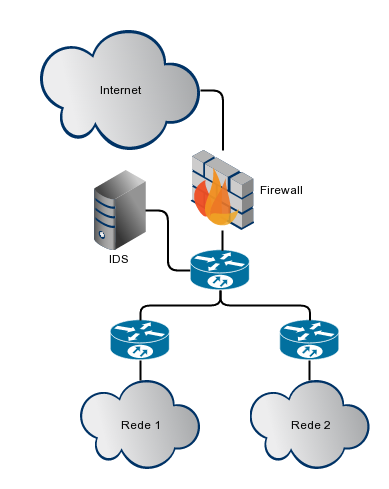
\includegraphics[height=7cm]{nids_passivo.png}
     \label{nids-passivo}
   }
   \quad
   \subfloat[NIDS Ativo]{
     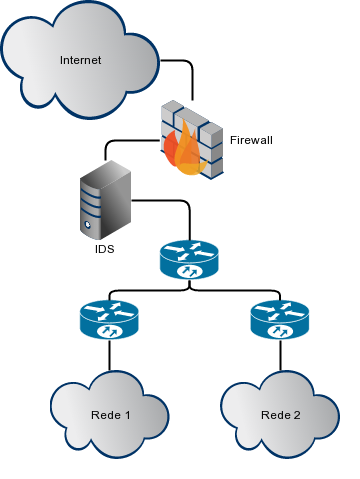
\includegraphics[height=7cm]{nids_ativo.png}
     \label{nids-ativo}
   }
   \caption{Exemplos de Arquitetura de NIDS}
   \label{nids}
  \end{figure}

 \section{Principais Ferramentas de IDS}
 \subsection{Snort}

 O Snort é um sistema de detecção e prevenção de intrusão de código fonte aberto escrita na linguagem de programação C bem conhecido pela comunidade da segurança da informação. Seu primeiro \textit{release} foi lançado em 1998 e desde então passa por constantes revisões e aperfeiçoamentos, com o passar dos anos se tornou o IDS mais utilizado no mundo. Ele combina análise baseada em assinaturas e anomalias, podendo operar em três modos: \textit{sniffer}, \textit{packet logger} e de sistema de detecção de intrusão (NIDS) \cite{snortorgbr}.

 No modo \textit{Sniffer}, o Snort captura os pacotes e exibi as informações no console. No modo \textit{Packet Logger}, além de capturar o tráfego, ele registrar essas informações em disco (arquivos de logs). E no modo NIDS, é o modo mais complexo, permite analise do pacotes de rede em tempo real.

 Existe quatro componentes no Snort: O \textit{Sniffer}, o Pré-processador, o Motor de Detecção e Módulo de Saída. Os componentes são organizados de acordo com a figura \ref{snort-componentes} \cite{kohlenberg2007snort}.

 \begin{figure}[!htb]
   \centering
   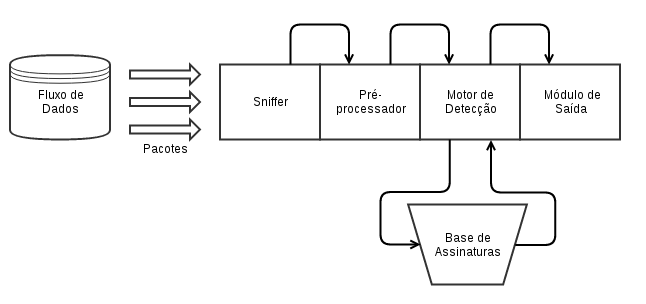
\includegraphics[scale=0.6]{snort_componentes}
   \caption{Componentes do Snort}
   \label{snort-componentes}
 \end{figure}

 \subsection{Suricata}
 \section{Conclusão}
 %Ex: Este capítulo apresentou...


